\documentclass[12pt]{report}
\usepackage{amsmath}
\usepackage{mathptmx}    % Times New Roman font
\usepackage{graphicx}    % For including images
\usepackage{ragged2e}    % For justification
\usepackage{setspace}    % For line spacing
\usepackage[margin=1in]{geometry} % 1-inch margins
\usepackage{titlesec}    % For customizing titles
\usepackage{fancyhdr}    % For customizing headers and footers
\setstretch{1.15}  % Word's default line spacing is approximately 1.15

% Adjust top margin and space above chapter titles
\setlength{\topmargin}{-0.5in}  % Adjust top margin (negative value reduces space)
\setlength{\headheight}{15pt}   % Adjust the height of the header
\setlength{\headsep}{20pt}      % Adjust the space between the header and text

% Customize chapter title spacing
\titleformat{\chapter}[display]
{\normalfont\huge\bfseries} % Format for the chapter title
{\chaptername\ \thechapter}{20pt}{\huge} % Spacing adjustments

% Define header
\fancyhf{}  % Clear all header and footer fields
\fancyhead[L]{\leftmark}  % Left-aligned header content
\fancyfoot[C]{\thepage}   % Centered page number at the bottom

% Remove horizontal lines in header and footer
\renewcommand{\headrulewidth}{0pt}  % No line at the top
\renewcommand{\footrulewidth}{0pt}  % No line at the bottom

% Apply the fancy header to all pages
\pagestyle{fancy}

\begin{document}
	\justifying
	
	\chapter*{Main Assignment (In lecture 3 pdf)}
	
	\section*{Questions}

	
	
	
	
	
	
	\subsection*{Question 1}
	A DC chopper with a resistive load of $R = 15 \ \Omega$ and an input voltage of $V = 250 \ \text{V}$ is considered. When the chopper is ON, its voltage drop is $3 \ \text{V}$, and the chopping frequency is $1.5 \ \text{kHz}$. Given that the duty cycle is 70%, determine the following:
	\begin{enumerate}
		\item Average output voltage
		\item RMS value of output voltage
		\item Effective input resistance of chopper
		\item Chopper output power
	\end{enumerate}
	
	\begin{center}
		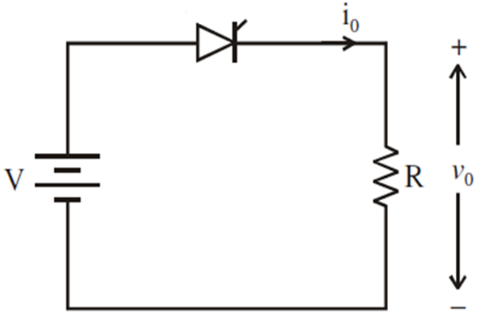
\includegraphics[width=0.4\textwidth]{Picture1.png}
		\\[1em]
		\textit{Figure 1: DC Chopper Circuit Diagram}
	\end{center}
	




     \subsubsection*{a) Average Output Voltage (\( V_{o,\text{avg}} \))}
     When the chopper is ON, the load voltage is given by:
     \[
     V_{\text{load, ON}} = V - V_{\text{drop}} = 250 \ \text{V} - 3 \ \text{V} = 247 \ \text{V}
     \]
     When the chopper is OFF, the load voltage is:
     \[
     V_{\text{load, OFF}} = 0 \ \text{V}
     \]
     Thus, the average output voltage is calculated as follows:
     \[
     V_{o,\text{avg}} = \alpha \times (V - V_{\text{drop}}) + (1 - \alpha) \times 0
     \]
     \[
     V_{o,\text{avg}} = 0.7 \times 247 + 0 = 172.9 \ \text{V}
     \]
     
     \subsubsection*{b) RMS Value of Output Voltage (\( V_{o,\text{rms}} \))}
     The RMS value of the output voltage is given by:
     \[
     V_{o,\text{rms}} = \sqrt{\alpha \times (V - V_{\text{drop}})^2}
     \]
     Substituting the values:
     \[
     V_{o,\text{rms}} = \sqrt{0.7 \times 247^2} = \sqrt{42,632.7} \approx 206.48 \ \text{V}
     \]
     
     \subsubsection*{c) Effective Input Resistance (\( R_{\text{eff}} \))}
     The effective input resistance of the chopper is calculated as:
     \[
     R_{\text{eff}} = \frac{R}{\alpha}
     \]
     Substituting the values:
     \[
     R_{\text{eff}} = \frac{15}{0.7} \approx 21.43 \ \Omega
     \]
     
     \subsubsection*{d) Chopper Output Power (\( P_o \))}
     Using the RMS voltage to calculate the output power:
     \[
     P_o = \frac{V_{o,\text{rms}}^2}{R}
     \]
     Substituting the values:
     \[
     P_o = \frac{(206.48)^2}{15} \approx 2,843.83 \ \text{W}
     \]
     Alternatively, using the average output voltage:
     \[
     P_o = \frac{V_{o,\text{avg}}^2}{R}
     \]
     \[
     P_o = \frac{(172.9)^2}{15} \approx 1,992.57 \ \text{W}
     \]
     The correct approach is to use the RMS value, thus:
     \[
     \boxed{P_o \approx 2,843.83 \ \text{W}}
     \]

	
	
	\subsection*{Question 2}
	An inverter supplies a 4-pole, three-phase induction motor rated at 220 V, 50 Hz. Determine the approximate output required of the inverter for motor speeds of:
	\begin{enumerate}
		\item[(i)] 950 rpm
		\item[(ii)] 1250 rpm
		\item[(iii)] 1550 rpm
		\item[(iv)] 1850 rpm
	\end{enumerate}
	
	
	For an inverter-fed induction motor, the output is controlled by varying the voltage and frequency simultaneously to maintain a constant V/f ratio. 
	
	\subsection*{Key Relationships}
	\begin{itemize}
		\item Synchronous speed: \( n_s = \frac{120 \times f}{P} \)
		\item Where \( f \) is the frequency, \( P \) is the number of poles.
		\item Synchronous speed \( = 1500 \, \text{rpm} \) for this 4-pole, 50 Hz motor.
	\end{itemize}
	
	\subsection*{Calculations for each speed}
	\begin{enumerate}
		\item[(i)] At 950 rpm:
		\begin{align*}
			\text{Desired speed:} & \quad 950 \, \text{rpm} \\
			\text{Required frequency:} & \quad \frac{950 \times 4}{120} = 31.67 \, \text{Hz} \\
			\text{Corresponding voltage:} & \quad \left(\frac{31.67}{50}\right) \times 220 \, \text{V} = 139.33 \, \text{V} 
		\end{align*}
		
		\item[(ii)] At 1250 rpm:
		\begin{align*}
			\text{Desired speed:} & \quad 1250 \, \text{rpm} \\
			\text{Required frequency:} & \quad \frac{1250 \times 4}{120} = 41.67 \, \text{Hz} \\
			\text{Corresponding voltage:} & \quad \left(\frac{41.67}{50}\right) \times 220 \, \text{V} = 183.33 \, \text{V}
		\end{align*}
		
		\item[(iii)] At 1550 rpm:
		\begin{align*}
			\text{Desired speed:} & \quad 1550 \, \text{rpm} \\
			\text{Required frequency:} & \quad \frac{1550 \times 4}{120} = 51.67 \, \text{Hz} \\
			\text{Corresponding voltage:} & \quad \left(\frac{51.67}{50}\right) \times 220 \, \text{V} = 227.33 \, \text{V}
		\end{align*}
		
		\item[(iv)] At 1850 rpm:
		\begin{align*}
			\text{Desired speed:} & \quad 1850 \, \text{rpm} \\
			\text{Required frequency:} & \quad \frac{1850 \times 4}{120} = 61.67 \, \text{Hz} \\
			\text{Corresponding voltage:} & \quad \left(\frac{61.67}{50}\right) \times 220 \, \text{V} = 271.33 \, \text{V}
		\end{align*}
		
	\end{enumerate}
	
	
	\subsection*{Question 3}
	The speed of a 15 hp, 250 V, 1300 rpm separately-excited DC motor is controlled by a single-phase fully-controlled full-wave rectifier bridge. The rated armature current is 40 A, with an armature resistance $R_a = 0.4 \ \Omega$, and the AC supply voltage is 270 V. The motor voltage constant is $K_e \Phi = 0.192 \ \text{V/rpm}$. Assume sufficient inductance is present in the armature circuit to make $I_a$ continuous and ripple-free:
	
	\begin{enumerate}
		\item[(a)] For $\alpha = 40^\circ$ and rated motor current, calculate the motor torque, motor speed, and supply power factor.
		\item[(b)] If the polarity of the armature emf is reversed (e.g., by reversing the field excitation), calculate the firing angle to keep the motor current at its rated value and the power fed back to the supply.
	\end{enumerate}
	
	
	
\section*{Part (a): For \(\alpha = 40^\circ\), Rated Motor Current}

\subsection*{Average Rectified Voltage}
\begin{align*}
	V_{avg} &= \frac{V_{ac}}{\pi} (1 + \cos \alpha) \\
	V_{avg} &= \frac{270}{\pi} (1 + \cos 40^\circ) \\
	V_{avg} &= \frac{270}{\pi} (1 + 0.766) \\
	V_{avg} &= 154.55 \, \text{V}
\end{align*}

\subsection*{Motor Speed}
\begin{align*}
	V_{avg} &= V_b + I_a R_a \\
	V_b &= K_e \Phi \times \text{Speed} \\
	154.55 &= 0.192 \times \text{Speed} + 16 \\
	\text{Speed} &= \frac{154.55 - 16}{0.192} \\
	\text{Speed} &= 1{,}450 \, \text{rpm}
\end{align*}

\subsection*{Motor Torque}
\begin{align*}
	T &= \frac{P}{\omega} \\
	T &= \frac{15 \times 746}{2 \pi \times \frac{1450}{60}} \\
	T &= 61.6 \, \text{Nm}
\end{align*}

\subsection*{Supply Power Factor}
\begin{align*}
	PF &= \cos(\alpha) \\
	PF &= \cos(40^\circ) \\
	PF &= 0.766
\end{align*}

\section*{Part (b): Reversed Armature EMF}

\subsection*{Average Rectified Voltage}
When polarity is reversed, the average voltage equation changes:
\begin{align*}
	V_{avg} &= \frac{V_{ac}}{\pi} (1 - \cos \alpha)
\end{align*}

\subsection*{Rated Current at 40A}
\begin{align*}
	154.55 &= \frac{270}{\pi} (1 - \cos \alpha) + 40 \times 0.4 \\
	\frac{270}{\pi} (1 - \cos \alpha) &= 138.55 \\
	1 - \cos \alpha &= \frac{138.55 \pi}{270} \\
	\cos \alpha &= 0.494 \\
	\alpha &= \arccos(0.494) \\
	\alpha &= 60^\circ
\end{align*}

\subsection*{Power Fed Back to Supply}
\begin{align*}
	P_{feedback} &= V_{ac} I_{avg} \cos \alpha \\
	I_{avg} &= \frac{2I_m}{\pi} (1 - \cos \alpha) \\
	I_{avg} &= \frac{2 \times 40}{\pi} (1 - 0.5) \\
	I_{avg} &= 25.46 \, \text{A} \\
	P_{feedback} &= 270 \times 25.46 \times \cos(60^\circ) \\
	P_{feedback} &= 3{,}300 \, \text{W}
\end{align*}
	
	
	\subsection*{Question 4}
	A separately excited DC motor with an armature resistance of $0.02 \ \Omega$ works on a DC supply of $230 \ \text{V}$. It draws an armature current of $150 \ \text{A}$ and its rated speed is $1500 \ \text{RPM}$. It is fed from a chopper controller for its motoring and braking operations. Assuming continuous conduction, calculate the duty ratio of the chopper at rated torque with a speed of $550 \ \text{RPM}$ during:
	\begin{enumerate}
		\item[(a)] Motoring
		\item[(b)] Braking
	\end{enumerate}
	
	
	
	Given:
	\begin{itemize}
		\item Supply Voltage (\( V \)) = 230 V
		\item Armature Resistance (\( R_a \)) = 0.02 \(\Omega\)
		\item Armature Current (\( I_a \)) = 150 A
		\item Rated Speed = 1500 RPM
		\item Speed at chopper operation = 550 RPM
	\end{itemize}
	

	\textbf{Voltage drop across armature:}	
	
	\[
	\text{Voltage drop across armature} = I_a \times R_a = 150 \times 0.02 = 3 \text{ V}
	\]	
	
	\textbf{At 1500 RPM, Back EMF (\( E_1 \)):}

	\[
	E_1 = V - (I_a \times R_a) = 230 - (150 \times 0.02) = 230 - 3 = 227 \text{ V}
	\]
	\subsection*{(a) Motoring Operation}
	\textbf{At 550 RPM, Back EMF (\( E_2 \))} can be calculated using proportional speed:
	\[
	E_2 = \left( \frac{550}{1500} \right) \times 227 = 83.17 \text{ V}
	\]
	\textbf{Duty Ratio for Motoring:}
	\[
	\text{Duty Ratio for Motoring} = \frac{E_2}{V} = \frac{83.17}{230} = 0.362 \text{ or } 36.2\%
	\]
	
	\subsection*{(b) Braking Operation}
	{In chopper braking, the motor acts as a generator.}
	
	
	\textbf{Back EMF during braking:}
	
	\[
	\text{Back EMF during braking} = V - (E_2 + \text{Voltage drop}) = 230 - (83.17 + 3) = 143.83 \text{ V}\]
	
	\textbf{Duty Ratio for Braking:}
	\[
	\text{Duty Ratio for Braking} = \frac{\text{Back EMF during braking}}{V} = \frac{143.83}{230} = 0.625 \text{ or } 62.5\%
	\]
	
	
	
	
	\subsection*{Question 5}
	A variable speed DC drive has a rated power of $15 \ \text{kW}$ and a rated speed of $1800 \ \text{rpm}$, driving a load that comprises a constant load of $T_L = 40 \ \text{Nm}$. The inertia of the drive system is $0.20 \ \text{kg} \cdot \text{m}^2$. Calculate the time taken to accelerate the load from zero to $900 \ \text{rpm}$, assuming the drive develops rated torque during the acceleration phase.
	
	
	
	
	
	
	
	
	
	\subsection*{Question 6}
	A series DC motor is to be controlled by a single-phase, half-controlled, full-wave rectifier bridge as shown below. The AC input voltage has an RMS value of $230 \ \text{V}$ at $50 \ \text{Hz}$. The combined armature and field resistance is $3.5 \ \Omega$ and inductance is $350 \ \text{mH}$. If the load torque is $40 \ \text{Nm}$ and damping is neglected, calculate the average current and the speed for $\alpha = 50^\circ$.
	
	\begin{center}
		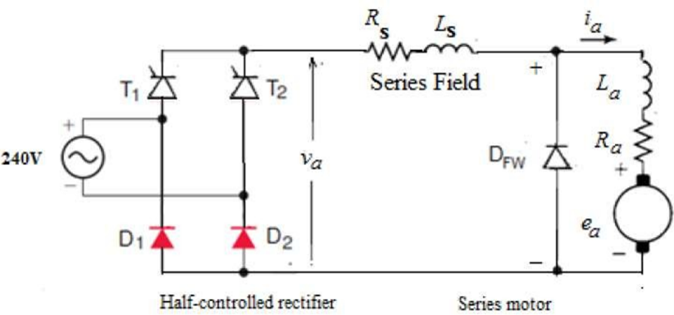
\includegraphics[width=0.4\textwidth]{Picture2.png}
		\\[1em]
		\textit{Figure 2: Series DC Motor Circuit Diagram}
	\end{center}
	
	
	
	\noindent For a single-phase half-controlled rectifier, the average output voltage is given by:
	\[V_{dc} = \frac{V_m}{\pi} (1 + \cos \alpha)\]
	where \(V_m = \sqrt{2} \times V_{rms} = \sqrt{2} \times 240 = 339.4\ \text{V}\). Substituting the values:
	\[V_{dc} = \frac{339.4}{\pi} (1 + \cos 60^\circ) = 162.1\ \text{V}\]
	
	\noindent The motor equation for a series DC motor is:
	\[V_{dc} = I_a (R_a + R_f) + K_{af} \times \omega \times I_a\]
	Substituting \(V_{dc} = 162.1\ \text{V}\), \(I_a \times R = I_a \times 2.5\ \Omega\), and \(K_{af} = 0.3\ \text{H}\):
	\[162.1 = 10 \times 2.5 + 0.3 \times \omega \times 10\]
	Simplifying:
	\[162.1 = 25 + 3\omega\]
	\[\omega = \frac{162.1 - 25}{3} = 45.7\ \text{rad/s}\]
	
	\noindent The torque equation is:
	\[T = K_{af} \times I_a^2\]
	Substituting \(T = 30\ \text{Nm}\) and \(K_{af} = 0.3\ \text{H}\):
	\[30 = 0.3 \times I_a^2 \implies I_a = \sqrt{\frac{30}{0.3}} = 10\ \text{A}\]
	
	\noindent Finally, the motor speed in rpm is:
	\[N = \frac{\omega \times 60}{2\pi} = \frac{45.7 \times 60}{2\pi} = 436.4\ \text{rpm}\]
	
	
	
	\subsection*{Question 7}
	Two three-phase induction motors are to be speed controlled by a cumulative cascade arrangement as shown in the figure below. The main motor has four poles, whereas the auxiliary motor has six poles. The supply voltage is $450 \ \text{V}$ and $50 \ \text{Hz}$ for the main motor, while the frequency in the rotor of the auxiliary motor is $1.5 \ \text{Hz}$. Calculate the slip of each motor and the combined speed of the whole set.
	
	\begin{center}
		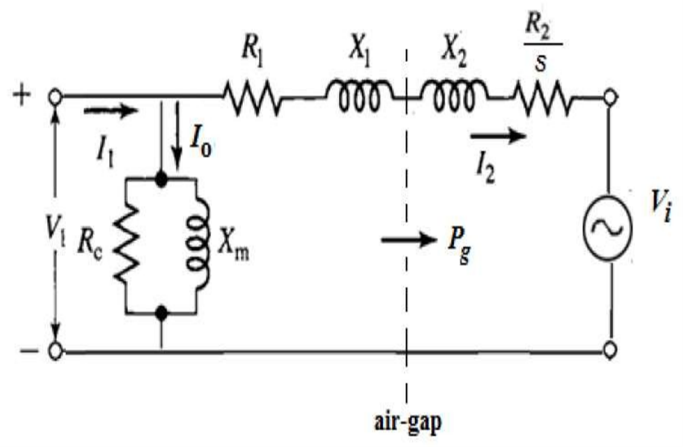
\includegraphics[width=0.4\textwidth]{Picture3.png}
		\\[1em]
		\textit{Figure 3: Cumulative Cascade Arrangement}
	\end{center}
	
	

	
\end{document}



